\contourlength{1.0pt}
\tikzset{>=latex} % for LaTeX arrow head

\colorlet{xcol}{blue!60!black}
\colorlet{myred}{red!85!black}
\colorlet{myblue}{blue!80!black}
\colorlet{mycyan}{cyan!80!black}
\colorlet{mygreen}{green!70!black}
\colorlet{myorange}{orange!90!black!80}
\colorlet{mypurple}{red!50!blue!90!black!80}
\colorlet{mydarkred}{myred!80!black}
\colorlet{mydarkblue}{myblue!80!black}
\tikzstyle{xline}=[xcol,thick]
\tikzstyle{Tline}=[line width=0.6]
\tikzstyle{width}=[{Latex[length=5,width=3]}-{Latex[length=5,width=3]},thick]
\def\tick#1#2{\draw[thick] (#1)++(#2:0.12) --++ (#2-180:0.24)}
\def\N{100} % number of samples

% HARMONIC OSCILLATOR FORCE


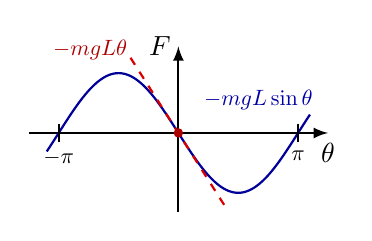
\begin{tikzpicture}
  \message{^^JHarmonic oscillation}
  \def\ymax{1.0}  % max y axis
  \def\xmax{1.9}  % max x axis
  \def\A{0.76}        % amplitude
  \def\T{(1.6*\xmax)} % period
  \draw[->,thick] (0,-\ymax) -- (0,1.1*\ymax) node[left=-1] {$F$};
  \draw[->,thick] (-\xmax,0) -- (\xmax,0) node[below] {$\theta$};
  \draw[xline,samples=100+\N,smooth,variable=\x,domain=-0.88*\xmax:0.88*\xmax]
    plot(\x,{-\A*sin(360/\T*\x)});
  \draw[xline,myred,dashed,samples=\N,smooth,variable=\x,domain=-0.20*\T:0.20*\T] %,line cap=round
    plot(\x,{-\A*2*pi/\T*\x});
  \fill[myred!80!black] (0,0) circle(0.06);
  \tick{{-\T/2},0}{90} node[below=0,scale=0.8] {$-\pi$};
  \tick{{ \T/2},0}{90} node[below=0,scale=0.8] {$\pi$};
  \node[mydarkblue,above left=0,scale=0.8] at (0.95*\xmax,0.25*\A) {$-mgL\sin\theta$};
  \node[mydarkred,above left=0,scale=0.8] at (-0.29*\xmax,1.1*\A) {$-mgL\theta$};
\end{tikzpicture}
